%% start of file `template.tex'.
%% Copyright 2006-2013 Xavier Danaux (xdanaux@gmail.com).
%
% This work may be distributed and/or modified under the
% conditions of the LaTeX Project Public License version 1.3c,
% available at http://www.latex-project.org/lppl/.


\documentclass[10pt,a4paper,sans]{moderncv}        % possible options include font size ('10pt', '11pt' and '12pt'), paper size ('a4paper', 'letterpaper', 'a5paper', 'legalpaper', 'executivepaper' and 'landscape') and font family ('sans' and 'roman')

% moderncv themes
\moderncvstyle{classic}                             % style options are 'casual' (default), 'classic', 'oldstyle' and 'banking'
\moderncvcolor{black}                               % color options 'blue' (default), 'orange', 'green', 'red', 'purple', 'grey' and 'black'
%\renewcommand{\familydefault}{\sfdefault}         % to set the default font; use '\sfdefault' for the default sans serif font, '\rmdefault' for the default roman one, or any tex font name
%\nopagenumbers{}                                  % uncomment to suppress automatic page numbering for CVs longer than one page

% character encoding
\usepackage[utf8]{inputenc}                       % if you are not using xelatex ou lualatex, replace by the encoding you are using
%\usepackage{CJKutf8}                              % if you need to use CJK to typeset your resume in Chinese, Japanese or Korean

% adjust the page margins
\usepackage[scale=0.75]{geometry}
%\setlength{\hintscolumnwidth}{3cm}                % if you want to change the width of the column with the dates
%\setlength{\makecvtitlenamewidth}{10cm}           % for the 'classic' style, if you want to force the width allocated to your name and avoid line breaks. be careful though, the length is normally calculated to avoid any overlap with your personal info; use this at your own typographical risks...

\usepackage{pdfpages}

% personal data
\name{Martin}{Ponce}
%\title{CV}                               		% optional, remove / comment the line if not wanted
\address{U2/93 Scarborough Beach Rd}{MT HAWTHORN WA 6016}{}% optional, remove / comment the line if not wanted; the "postcode city" and and "country" arguments can be omitted or provided empty
\phone[mobile]{+61 416 357 709}                   % optional, remove / comment the line if not wanted
%\phone[fixed]{+2~(345)~678~901}                    % optional, remove / comment the line if not wanted
%\phone[fax]{+3~(456)~789~012}                      % optional, remove / comment the line if not wanted
\email{martin.ponce@outlook.com}                               % optional, remove / comment the line if not wanted
%\homepage{www.johndoe.com}                         % optional, remove / comment the line if not wanted
%\extrainfo{additional information}                 % optional, remove / comment the line if not wanted
%\photo[64pt][0.4pt]{picture}                       % optional, remove / comment the line if not wanted; '64pt' is the height the picture must be resized to, 0.4pt is the thickness of the frame around it (put it to 0pt for no frame) and 'picture' is the name of the picture file
%\quote{Some quote}                                 % optional, remove / comment the line if not wanted

% to show numerical labels in the bibliography (default is to show no labels); only useful if you make citations in your resume
%\makeatletter
%\renewcommand*{\bibliographyitemlabel}{\@biblabel{\arabic{enumiv}}}
%\makeatother
%\renewcommand*{\bibliographyitemlabel}{[\arabic{enumiv}]}% CONSIDER REPLACING THE ABOVE BY THIS

% bibliography with mutiple entries
%\usepackage{multibib}
%\newcites{book,misc}{{Books},{Others}}
%----------------------------------------------------------------------------------
%            content
%----------------------------------------------------------------------------------
\begin{document}

%-----       letter       ---------------------------------------------------------
% recipient data
\recipient{Bankwest}{108 St. Georges Tce\\PERTH 6000 WA}
\date{\today}
\opening{Dear Sir or Madam,}
\closing{Sincerely,}
\enclosure[Attached]{Resume and transcript}          % use an optional argument to use a string other than "Enclosure", or redefine \enclname
\makelettertitle

I am writing with interest regarding the ``Java API Developer'' position advertised on \href{https://www.seek.com.au/job/33237951?type=standout&tier=no_tier&pos=1&whereid=3000&userqueryid=9ed0336a00786a41bf4398256cfb67a3-2819278&ref=beta}{Seek.com.au}. I am mature age student, in my third and final year of studying Bachelor of Computer Science at Edith Cowan University, majoring in Software Engineering and recently spent 18 months at IBM as a Software Developer Intern where I worked on real commercial products.

I have a passion for writing code and problem solving and my ultimate goal is to pursue a long lasting career in the software development industry. I've had a taste of what it's like in the industry for the last 18 months and I have met all demands and challenges head on with enthusiasm and a thirst for learning.

During my time at IBM, I was involved with two projects. The first was z Operational Insights (zOI) where myself and another intern developed additional proof of concept insights. This project involved adding new features to analyse a new subset of log records in a Java 8 based backend which then provided REST API endpoints so that the Angular 1 based frontend could request the analysis output in JSON format. I was also involved in developing new views for these outputs, using Angular 1 and D3.js to visualize the data.

The second project was Common Data Provider for z Systems (CDPz), where I spent the majority of my time at IBM. My responsibility was to develop a Java 7 based component called the Data Streamer that accepted log records from multiple gatherers over TCP/IP, process that data, then send it on to multiple subscribers, also via TCP/IP. As well as development code, all classes and methods were delivered with corresponding unit tests and I was also involved in code reviews. In addition to development, I was also involved in writing documentation for features I developed which were included in the user manual. I was given the responsibility to design some aspects of the Data Streamer, and became regarded as one of the main developers, even though I was only an intern.

Although the projects I have been involved with did not provide any experience with databases, I have scored well (96 HD) in the Systems and Database Design unit at ECU, and have a solid grasp of the fundamentals of relational database design and implementation.

While I have yet to complete my degree, I believe that my demonstrated initiative, passion for software development and willingness to learn and share knowledge makes me a worthy candidate for the position, and plan to complete my degree by studying part time if successful in securing the role.

%I am an Australian citizen, and can provide proof of citizenship at your request. I work diligently at university which is proven by my current weighted average mark of 85.38 HD. Please find a transcript attached with this document. I have previously worked as a junior business analyst at Synergy for 12 months which provided some insight into the development lifecycle. I am also fluent in English, having excellent written and spoken communication skills.

Please find my resume and current course transcript attached below. I appreciate your consideration for the role.

%Regards,\\
%Martin Ponce

\makeletterclosing

\clearpage

%\begin{CJK*}{UTF8}{gbsn}                          % to typeset your resume in Chinese using CJK
%-----       resume       ---------------------------------------------------------
\makecvtitle

\section{Education}
\cventry{2014--Present}{Bachelor of Computer Science}{Edith Cowan University}{Perth}{}{Current WAM Average: 83.23 HD\newline
Major: Software engineering\newline
Year: Third year student}  % arguments 3 to 6 can be left empty

\cventry{2002--2004}{Graphic Design Diploma}{KvB Institute of Technology}{North Sydney}{}{WAM Average: 73.46 CR\newline
Print and digital media}

\section{Experience}
%\subsection{Vocational}
% IBM
\cventry{2016--2017}{Software Developer Intern}{IBM}{Perth}{}{Due to my high distinction grade average, I was invited to take part in ECU's Work Integrated Learning program, and applied for an internship role at IBM. During my internship, I was heavily involved in the development of a new commercial product and gained valuable experience working in a professional environment where my knowledge, technical and interpersonal skills were put to the test in a software developer role.\newline
\newline{Responsibilities:}
\begin{itemize}
\item Initially worked on developing additional proof of concept features for \href{http://www-03.ibm.com/software/products/en/z-oi}{z Operational Insights}
	\begin{itemize}
	\item An existing web application based on Angular 1 delivering system insights based on user uploaded log records
	\item Developed additional analytic calculations in Java backend with REST API endpoints to deliver insight data to Angular 1 based frontend
	\item Frontend presents data with graphs and charts, gained experience in using charting library D3.js
	\end{itemize}
\item During the majority of my internship, I was involved in the development of a greenfield project called \href{http://www-03.ibm.com/software/products/en/common-data-provider}{Common Data Provider for z Systems}
	\begin{itemize}
	\item The product gathers log records from multiple sources in a z/OS system, processes the data and forwards them to multiple subscribers through a single interface
	\item I was responsible for the development of the Java based Data Streamer component of the product, which accepts log records from independent log gatherer components, processes the data and forwards them to subscribers over TCP sockets
	\item Development time for initial release was in a very short timeframe, and proved my time management skills and ability to work under pressure by delivering expectations at the end of every sprint
	\item Code commits were accompanied by unit tests for each class and method, using JUnit and Mockito frameworks
	\item I was involved in developing the Data Streamer build and test automation Gradle scripts
	\item I was also responsible for writing user documentation for any features that I developed which were included in the manual
	\item My team consisted of fellow interns and a graduate, quickly becoming the person the other interns could turn to and depend on for assistance
	\item I also demonstrated an eagerness to learn from others, being fully aware that I was surrounded by developers with years of experience and soaked in as much knowledge from them as possible by asking questions, learning from and being open to productive criticism and building quality relationships with them
	\end{itemize}
\end{itemize}}
% Synergy BA
\cventry{2012--2013}{Junior Business Analyst}{Synergy}{Perth}{}{Gained experience as a junior business analyst for Synergy's Continuous Improvement department for 12 months, working closely with the Billing Services department to improve current business processes.\newline
\newline{Responsibilities:}
\begin{itemize}
\item Developed Standard Operating Procedures and training material for Billing Services users of Synergy's SAP ISU system
\item Assisted in identifying opportunities where business processes could be improved
	\begin{itemize}
	\item Developed
		\begin{itemize}
		\item BPMN process models of current and proposed processes
		\item Business Requirements documents
		\item Change request documents
		\end{itemize}
	\end{itemize}
\item Performing and writing User Acceptance tests for proposed changes to Synergy's SAP system
\item Was involved in development and testing of new SAP security roles for all members of the Billing Services department ahead of a major system upgrade
\end{itemize}}
% Synergy BPEMO
\cventry{2008--2012}{Billing Process Exceptions Management Officer}{Synergy}{Perth}{}{Resolved technical billing exceptions in Synergy's Billing Services department.\newline
\newline{Responsibilities:}
\begin{itemize}
\item Resolved technical billing issues using Synergy's SAP system, by analysing basic and interval meter readings
\item Received awards in recognition of my deep knowledge and understanding of business processes and market rules, balancing business needs and impact to customer experience
\item I was made responsible for escalated enquiries, where difficult, unresolved issues were logged and required attention from a knowledgeable and customer focused employee which may potentially result in a customer complaint
\item I was involved in analysing the escalated enquiries log to identify gaps in training and made recommendations to update Standard Operating Procedures to reduce escalated enquiries
\item I provided support for my colleagues when they faced complex issues, provided coaching and mentored new team members
\item I was proactive in QA and provided helpful feedback when errors were encountered, and often filled in for leadership roles when required
\end{itemize}}


\section{Relevant skills}
\cvitem{Basic}{JavaScript, C\#, ASP.NET MVC, PHP, SQL, Gradle}
\cvitem{Intermediate}{Java, ASP.NET MVC, HTML, CSS, Git, MS Project, Linux CLI \& scripting}
\cvitem{Advanced}{MS Visio, Adobe Creative Suite}

\section{Interests}
\cvitem{}{Basketball, weekly team competition}
\cvitem{}{Electronic music production}
\cvitem{}{PC gaming}

%\clearpage\end{CJK*}                              % if you are typesetting your resume in Chinese using CJK; the \clearpage is required for fancyhdr to work correctly with CJK, though it kills the page numbering by making \lastpage undefined

\clearpage

\section{Transcript as of April 2017}

\vspace{2em}

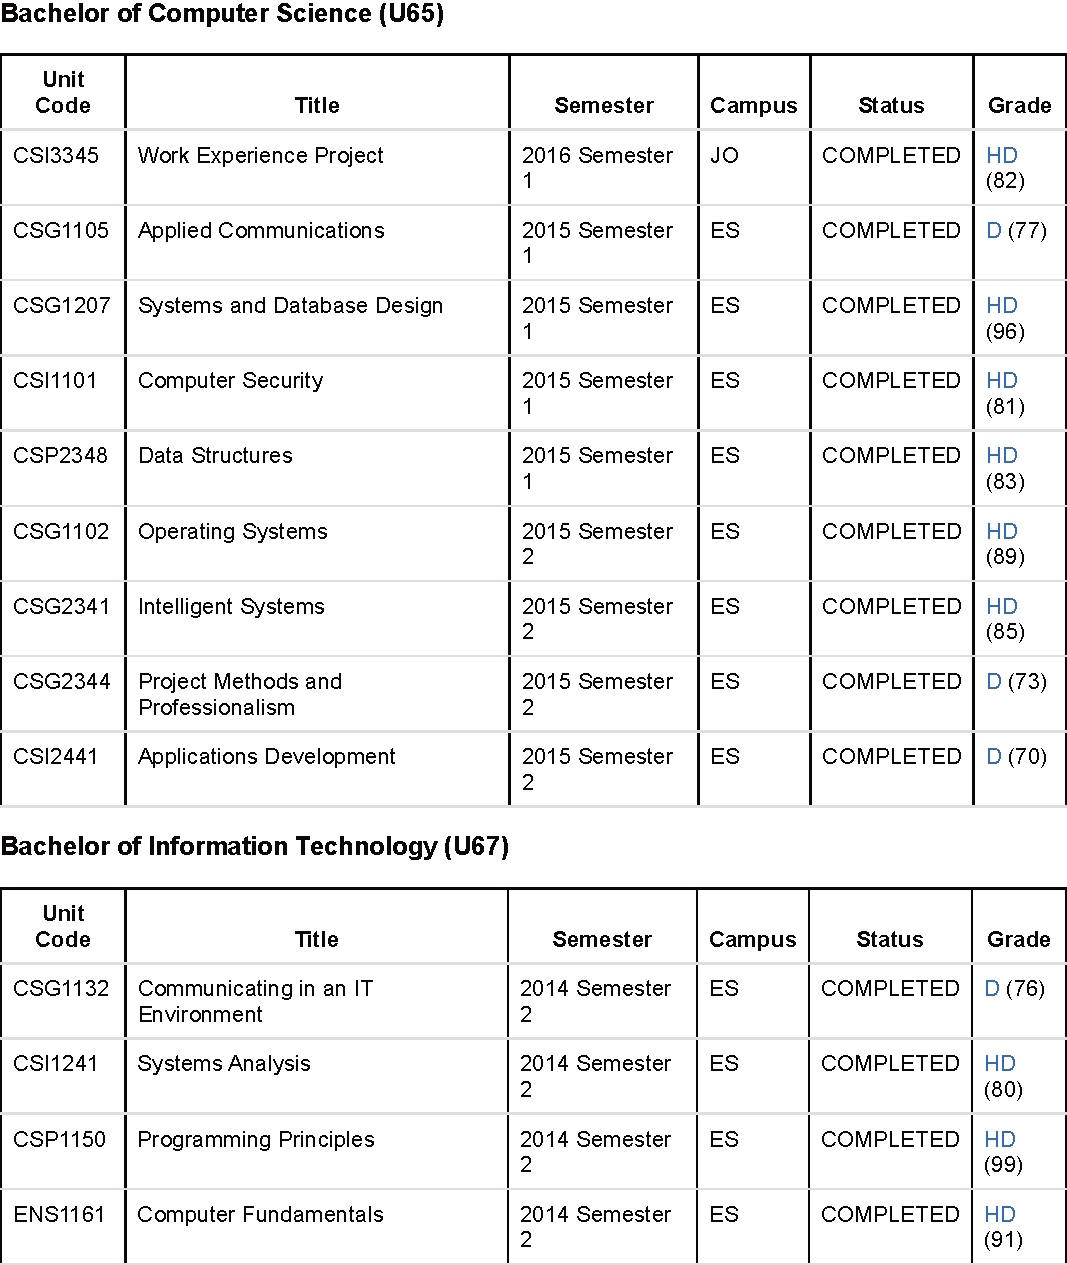
\includegraphics[scale=.8]{./img/Transcript.pdf}


\end{document}


%% end of file `template.tex'.
